\chapter{Tex-Demo}

This chapter has a bunch of random \LaTeX\  examples. If you are reading this in the final version, hi. This is a bit awkward.



Here you see me cite stuff \cite{fma_dataset}. Add new stuff to cite from to 'literature.bib' and ignore the stuff already in there, thats just for copy-pasting (and I will delete it later, probably).

Here is an image. Delete the [!htb] if you don't need the image anywhere close by, and \LaTeX\  will store it somewhere on the dark side of the moon.
\begin{figure}[!htb]
	\centering
	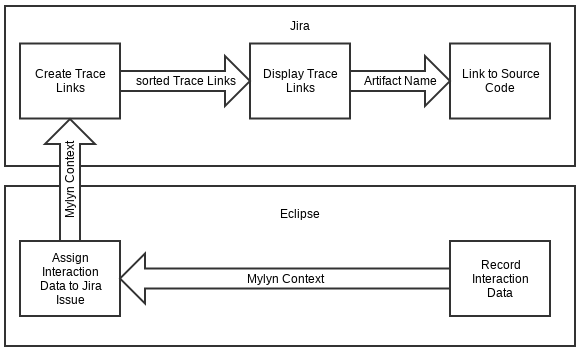
\includegraphics[width=.9\linewidth]{images/Approach-Flowchart.png}
	\caption{Some random image I had lying around in another \LaTeX\  report.}
	\label{fig:random_image}
\end{figure}

Here is me talking about figure \ref{fig:random_image}.

\begin{figure}[!htb]
	\centering
	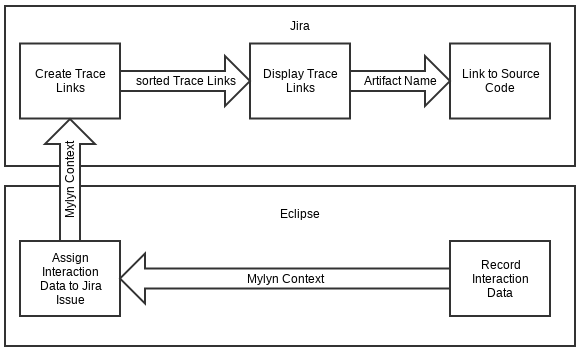
\includegraphics[width=.4\linewidth]{images/Approach-Flowchart.png}
	\quad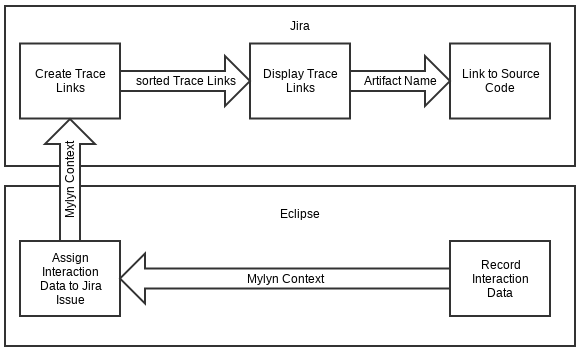
\includegraphics[width=.4\linewidth]{images/Approach-Flowchart.png}
	\caption{This is getting out of hand! Now there is two of them!}
	\label{fig:lolnooneevenusesthisimage}
\end{figure}


Look at table \ref{tab:somerandomtablethatshouldnotbehere}, it's all shiny and without lines boxing it in on all sides. Or you can just draw a sudoku, see if I care.


\begin{center}
\begin{tabular}{ p{\textwidth /4}  p{\textwidth *3 /5 }}

	Description & The way developers approach a task can provide detailed information about the structure of the project they are working on.
	Using this knowledge, other team-members can familiarize themselves with new parts of the project faster.
	This information can be displayed as trace links, which show the source code entities, that are relevant to a particular requirement specification.
	While the users can benefit from these trace links, their creation should not interfere with the normal workflow. Why is this even still on my hard-drive, I handed it in years ago.\\
	\hline
	User Subtasks & User Subtask 1.1: perform interactions\\
	& User Subtask 1.2: commit changes related to an issue\\
	& User Subtask 1.3: browse linked code entities\\	
\end{tabular}
	\label{tab:somerandomtablethatshouldnotbehere}
\captionof{table}{If you don't add a caption, the table wont show up in the list of tables. I invested a lot of clicks into making that, so you better think of something clever to put there.}
\end{center}

Notice how this tabular doesn't float all over the place? use regular tables if you prefer it that way.